\documentclass[12pt]{article}
\usepackage{listings}
\usepackage{amssymb}
\usepackage{amsthm}
\usepackage{amsmath}
\usepackage{graphicx}
\usepackage{subfig}
\usepackage{multirow}
\usepackage{float}
\usepackage{fancyhdr}
\usepackage{caption, subcaption}
\usepackage{tabularx}
\usepackage{booktabs}
\usepackage{multicol}
\usepackage{array}
\usepackage{adjustbox}
\usepackage[cache=false]{minted}
\usepackage{xcolor}
\usepackage[font=small]{caption}
\usepackage{siunitx}
\usepackage{subfigure}
\usepackage{subcaption}
\usepackage{graphicx} % Include this line in the preamble

\definecolor{bg}{rgb}{1.0, 0.97, 0.7} % Light yellow

\setminted[c]{
  bgcolor=bg,
  linenos,
  fontsize=\footnotesize,
  breaklines
}

\captionsetup{compatibility=false}
\usepackage[hidelinks, colorlinks=true, linkcolor=black, urlcolor=blue, citecolor=red]{hyperref}
%margin settings
\usepackage[left=2.5cm, right=2.5cm, top=4cm, bottom=3cm, footskip=0.5cm]{geometry}
% suppressing page numbers
\renewenvironment{abstract}
{\quotation
  {\large\bfseries\abstractname\centering\par\noindent\rule{\linewidth}{.5pt}\medskip}
  \noindent}
{\par\noindent\rule{\linewidth}{.5pt}\endquotation}

% Make headers
\usepackage{fancyhdr}
\pagestyle{fancy}
\fancyhf{}
\fancyhfoffset[L]{1cm} % left extra length
\fancyhfoffset[R]{1cm} % right extra length
\rhead{Group: 1}
\lhead{HW 04: Parallelization of One Dimensional Diffusion Equation Solver }
\fancyfoot[C]{\thepage}


\lstset{frame=tb,
  language=C,
  aboveskip=3mm,
  belowskip=3mm,
  showstringspaces=false,
  columns=flexible,
  basicstyle={\small\ttfamily},
  numbers=none,
  numberstyle=\tiny\color{red},
  keywordstyle=\color{blue},
  commentstyle=\color{green},
  stringstyle=\color{red},
  breaklines=true,
  breakatwhitespace=true,
  tabsize=3
}
\title{Homework 04\\ Parallelization of One Dimensional Diffusion Equation Solver}
\date{\today}
\author{Enes Çağlar Korkmazgöz 2370567 - Hasan Kaan Özen 2378586}

\begin{document}
\maketitle
\begin{abstract}
In this report, parallelization implementation and results of a one-dimensional diffusion equation solver are presented. Two different parallel configurations are compared, one containing MPI and one containing OpenMP. Strong scaling analysis and run time results are presented and discussed. These results show that the run times of MPI implementation are smaller than the run times of OpenMP implementation, where the differences appear clearer as the resolution increases. However, at some point, when the number of processes exceeds a certain number, the decrease in run time does not change significantly. Consequently, the total power consumption should be considered since it is a major parameter in modern HPC systems.
\end{abstract}
\newpage
\tableofcontents
\newpage
\section{Introduction}
\noindent
Parallel computing creates many options in the field of scientific computing to decrease total run times which directly relates to computational cost. Problems may become large enough for a simulation to take weeks to complete. Without parallel computing, problems are compiled by a single processor, even when other processors are available. The utilization of parallel computing creates a distributed workflow between the allocated processors. With the right implementations, the total run times significantly decrease. In this report, an explicit in-time one-dimensional finite difference solver for the diffusion equation which is presented on Equation \ref{eq:1} is parallelized using MPI(Message Passing Interface) and OpenMP(Open Multi-Processing). The implementations of these methods are provided in detail, followed by results of total run times and a scaling analysis. The findings are then discussed and interpreted under rational arguments.



\begin{equation}
\label{eq:1}
    \frac{\partial q}{\partial t} = \nabla \cdot (k\nabla q) + f(x,t)
\end{equation}
%%%%%%%%%%%%%%%%%%%%%%%%%%%%%%%%%%%%%

\section{Understanding The Solver}
\label{sec:2}
 The solver is an explicit in-time solver that initializes the field variable according to initial and boundary conditions. Then, the Forward Euler method is applied with central differencing to solve the field variable at the next time step. The central differencing method is presented in Equation \ref{eq:2} and the Forward Euler method is presented in Equation \ref{eq:3} where q stands for the field variable, k stands for the diffusion coefficient and f is the source function.
 \begin{equation}
 \label{eq:2}
\nabla \cdot (k\nabla q) + f(x, t) \approx rhs(q, t) = \frac{k}{dx^2} (q_{i-1} - 2q_i + q_{i+1}) + f(x_i, t)
\end{equation}
\begin{equation}
\label{eq:3}
    q(x, t + dt) = q(x, t) + dt \times {rhs}(q, t).
\end{equation}
Observing the equations, it is evident that the program contains nodal computation looping with time. MPI can be utilized to create communications between processors and OpenMPI can be utilized for the parallelization of the computations.
\section{Implementation Details}
\begin{table}[H]
\centering
\caption{Processor Specs}
\begin{tabular}{lc}
\toprule
\textbf{Specification} & \textbf{Details} \\
\midrule
Product & Intel i7-12650H \\
Total Cores & 10 \\
Performance Cores & 6 \\
Efficient Cores & 4 \\
Total Threads & 16 \\
Base Frequency & 1 GHz\\
Max Turbo Frequency & 4.7 GHz \\
Cache & 24 MB \\
\bottomrule
\end{tabular}
\end{table}
\subsection{MPI}
The utilization of MPI begins with assigning a number of nodes to each processor that is utilized. This directly controls the resolution of the mesh. Since every processor will deal with a number of nodes, a communication algorithm must be initialized. Because the solver is a one-dimensional solver, communication implementation is required for the first and last nodes of the processors. This is achieved by creating shadow nodes that are only utilized for sending and receiving data. The illustration of the algorithm is presented in Figure \ref{fig:1}. The implementation details are presented below. The code checks if the node of interest is on the boundary by checking the rank on an if statement. Since this is a one-dimensional problem, only the first node of the first rank and the last node of the last rank are boundaries. Thus, with the implemented if statements, these nodes are excluded from the communication algorithm. The communications are done with MPI\textunderscore{}Recv and MPI\textunderscore{}Send syntaxes. After creating the communication algorithm, every rank processes the necessary computations on their assigned nodes.
To compile the file, use the following in the terminal:\\
\texttt{mpicc -o heat1d heat1d.c -lm}
To run the file, use the following in the terminal:\\
\texttt{mpirun -np num\_of\_processes ./heat1d num\_of\_nodes\_per\_process}\\

\begin{figure}[H]
\centering
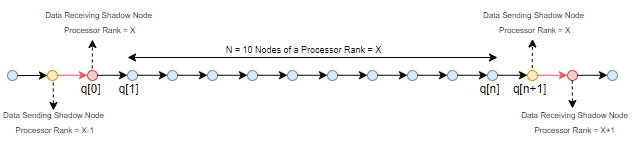
\includegraphics[width=\textwidth]{mpi_algo.png}
\caption{The utilized MPI algorithm.}
\label{fig:1}
\end{figure}

\begin{itemize}
    \item Compute coordinates of the nodes. The loop starts from 1 and goes to n which is the last node. This is because the coordinates of the shadow nodes at i=0 and i=n+1 are not important.
    \begin{minted}[linenos,breaklines,bgcolor=bg]{c}
    for ( int i = 1; i <= n; i++ ){
        x[i] = (double)(x_min + (dx*((rank * n) + i - 1)));
    \end{minted}
    \item Implement MPI communication structure. This communication assigns q values to the shadow variables so that they can be used as the next or previous data points in the Forward Euler method presented in the following item.
\begin{minted}[linenos,breaklines,bgcolor=bg]{c}
//Define binary communication directions since the problem is 1D.
  int leftcomms= 0;
  int rightcomms = 1;
  for (int step = 1; step <= Nsteps; step++) {
    double time_new = time + step*dt; 
    ////Create the communications by setting if conditions to exclude boundary nodes.
    // Check if rank=0 since the first node of rank(0) is boundary.
    if ( rank > 0 ) {
    //Send the information from the first node(1) of the ongoing rank to the last ghost node(n+1) of the previous rank.
        MPI_Send ( &q[1], 1, MPI_DOUBLE, rank-1, leftcomms, MPI_COMM_WORLD );
    //Receive the information from the previous rank to the first ghost node(0) of the ongoing rank..
        MPI_Recv ( &q[0], 1, MPI_DOUBLE, rank-1, rightcomms, MPI_COMM_WORLD, &status );}
    //Check if rank=size-1 since the last node of rank(size-1) is boundary.
    if ( rank < size-1 ) {
    //Receive the information from the next rank to the last ghost node(n+1) of the ongoing rank.
        MPI_Recv ( &q[n+1], 1,  MPI_DOUBLE, rank+1, leftcomms, MPI_COMM_WORLD, &status );
    //Send the information from the last node(n) of the ongoing rank to the first ghost node(0) of the next rank.
        MPI_Send ( &q[n], 1, MPI_DOUBLE, rank+1, rightcomms, MPI_COMM_WORLD );}
\end{minted}
    \item Compute the field variable at the next time point. This is done by implementing the right-hand side function on Equation \ref{eq:2} in the Forward Euler method in Equation \ref{eq:3}. In the for loop, n stands for the number of nodes of each processor Afterwards, the boundary nodes of first and last ranks are updated according to the boundary condition with respect to time.
    \begin{minted}[linenos,breaklines,bgcolor=bg]{c}
    for (int step = 1; step <= Nsteps; step++) {
        double time_new = time + step*dt; 
        for (int i = 1; i <= n; i++) {
            qn[i] = q[i] + dt * ((k / (dx * dx)) * (q[i - 1] - 2.0 * q[i] + q[i + 1]) + source(x[i], time));}
        if (rank==0){
          qn[1] = boundary_condition ( x[1], time_new );
        }
        if (rank == size - 1 ){
          qn[n] = boundary_condition ( x[n], time_new );
        }
    \end{minted}
    \item Update the field variable information at nodes with the new value.
    \begin{minted}[linenos,breaklines,bgcolor=bg]{c}
    for (int i = 1; i <= n; i++) {
        q[i] = qn[i];
    }
    \end{minted}
\end{itemize}
\subsection{OpenMP}
The OpenMP implementation is done on two functions in the solver. These functions are the computation function of the field variable for the next time point, and the update function of the next time point to the field variable array. The implementation details are presented below.
\begin{itemize}
\item Compute coordinates of the nodes. Now the for loop starts from i=0 to n-1. Different from the MPI version, the n stands for the total number of nodes in the domain, and x[n-1] is the last node. Moreover, the variable i starts from zero because there is no shadow variable in this program. After all, OpenMP manages the communications at parallelization.
    \begin{minted}[linenos,breaklines,bgcolor=bg]{c}
  for ( int i = 0; i < n; i++ ){
    x[i] = (double)(x_min + (dx*i));}
    \end{minted}
    \item Compute the field variable at the next time point. This is done by implementing the right-hand side function on Equation \ref{eq:2} in the Forward Euler method in Equation \ref{eq:3}. Afterwards, the global left and global right nodes which are boundary nodes are updated according to the boundary condition with respect to time.
    \begin{minted}[linenos,breaklines,bgcolor=bg]{c}
    for (int step = 1; step <= Nsteps; step++) {
        double time_new = time + step*dt; 
        #pragma omp parallel for
        // compute q values at all nodes except boundaries
        for (int i = 1; i < n-1; i++) {
            qn[i] = q[i] + dt*((k/(dx*dx)*(q[i-1]-(2*q[i])+q[i+1])) + source(x[i],time));
        }
        // update boundaries
        qn[0] = boundary_condition(x[0], time_new);
        qn[n-1] = boundary_condition(x[n-1], time_new);}
    \end{minted}
    \item Update the field variable array with the new value.
    \begin{minted}[linenos,breaklines,bgcolor=bg]{c}
    #pragma omp parallel for
    for (int i = 0; i < n; i++) {
        q[i] = qn[i];
    }
    \end{minted}
\end{itemize}
\noindent
To compile the file, use the following in the terminal:\\
\texttt{gcc -fopenmp -o heat1d\_omp heat1d\_omp.c -lm}\\
To run the file, use the following in the terminal:\\
\texttt{./heat1d\_omp domain\_per\_core num\_of\_cores}\\
\newpage
\section{Discussion and Results}
The Tables \ref{tab:n2400}, \ref{tab:n3000}, and \ref{tab:n6000} show that as the problem domain size increases (i.e. the resolution), the effects of MPI becomes more dominant over OpenMP. However, for small sized problems the difference between those two is not significant and implentation of MPI is more difficult than the implementation of OpenMP. Moreover, as number of processes increases in a MPI, the power consumption becomes greater as a consequence.\\
These result should not be a conclusion as MPI models are generally preferred in HPC systems as these utilize distributed memory approach whilst OpenMP is more suitable for modern computers, not for HPC systems.\\
Also there are other factors affecting the overall system performance and hence the tabulated results, the system condition. As we test the codes generated, our computers were also working on other tasks and running other apps. At some points (especially for when the process or core number reaches 6) the idle time of that processor becomes more dominant over other processes as there needs to be enough cores to run the OS and other apps.
\begin{table}[h!]
\centering
\caption{Computational performance comparison between MPI and OpenMP\\ Total Nodes: 2400}
\resizebox{\textwidth}{!}{
\label{tab:n2400}
\begin{tabular}{ccccc}
\hline
\multicolumn{2}{c}{MPI} & \multicolumn{3}{c}{OpenMP} \\
\hline
Num of Process & Time Taken (s) & Num of Cores & Time Taken (s) & Computation Load per Process/Core \\
\hline
2 & 2.777713 & 2 & 3.524228 & 1200 \\
4 & 1.959753 & 4 & 2.300896 & 600 \\
6 & 1.982581 & 6 & 2.147756 & 400 \\
\hline
\end{tabular}
}
\label{tab:my_label}
\end{table}


\begin{table}[h!]
\centering
\caption{Computational performance comparison between MPI and OpenMP\\ Total Nodes: 3000}
\resizebox{\textwidth}{!}{
\label{tab:n3000}
\begin{tabular}{ccccc}
\hline
\multicolumn{2}{c}{MPI} & \multicolumn{3}{c}{OpenMP} \\
\hline
Num of Process & Time Taken (s) & Num of Cores & Time Taken (s) & Computation Load per Process/Core \\
\hline
2 & 4.996306 & 2 & 7.218197 & 1500 \\
4 & 3.430658 & 4 & 4.175756 & 750 \\
6 & 3.335853 & 6 & 3.713506 & 500 \\
\hline
\end{tabular}
}
\label{tab:my_label}
\end{table}

\begin{table}[h!]
\centering
\caption{Computational performance comparison between MPI and OpenMP\\ Total Nodes: 6000}
\resizebox{\textwidth}{!}{
\label{tab:n6000}
\begin{tabular}{ccccc}
\hline
\multicolumn{2}{c}{MPI} & \multicolumn{3}{c}{OpenMP} \\
\hline
Num of Process & Time Taken (s) & Num of Cores & Time Taken (s) & Computation Load per Process/Core \\
\hline
2 & 42.506725 & 2 & 51.779862 & 3000 \\
4 & 24.74689 & 4 & 29.275777 & 1500 \\
6 & 24.257124 & 6 & 26.61659 & 1000 \\
\hline
\end{tabular}
}
\label{tab:my_label}
\end{table}







%%%%%%%%%%%%%%%%%
\clearpage

\section{Conclusion}
In this project, it is seen that MPI is an efficient way of solving large problems. Although its implementation is more difficult than implementation of OpenMP, it has wider range of working areas (in modern HPC systems as it uses a distributed memory system) yet OpenMP is limited with shared memory system. In the codes provided, a point-to-point communication is used for memory transfer across different processes for MPI implementation. Moreover, in the Figure \ref{fig:1} it is shown that the algorithm is based on transferring information from one process to another by using shadow nodes to use memory allocations efficiently and to make the code as fast as possible.\\
From the strong-scale analyses it is shown that as the number of process used by the computer is increased, the computational time decreased drastically and hence yielded a better performance. But one should be careful that as the number of process increases, the performance parameter does not always increase. This is due to the delay when different processes passes information from one to another. As this effect becomes more dominant over the work-load decrease corresponding more processes, the efficiency starts decreasing and hence is limited at some point. There are specific models related determining this performance criteria (i.e. Amdahl and Gustafson) and they use different mathematical models to measure performance characteristics of the system. Moreover, one should also be careful that there are many ways to deviate from the actual performance by using wrong scalings as mentioned in the Lecture Notes Part 7 [1]. \\
OpenMP, on the other hand, lacks performance when compared against the MPI. The reason is OMP uses shared memory approach and also it is restricted by the omp provider how the domain is shared across cores. It would be also a good idea to combine MPI and OpenMP with their strengths, combining both shared and distributed memory approaches.\\
Additionally, energy consumption is an emerging topic in the real-world in modern HPC systems. As number of processes increase, it directly affects the power consumption hence it is also a decision factor when comparing MPI and OpenMP.\\
In conclusion, while MPI boasts superior scalability and flexibility in distributed environments, OpenMP's shared memory model provides a more accessible entry point for parallelization. The choice between MPI and OpenMP—or a hybrid of the two—should be informed by the specific requirements of the task, including the scale of the problem, the available hardware, and the desired balance between computational performance and energy efficiency.
\noindent

\newpage
\section{References}
[1] Lecture notes of Ali Karakuş for ME489.


\end{document}